\section{Our approach}

\begin{figure}[htbp]
\begin{center}
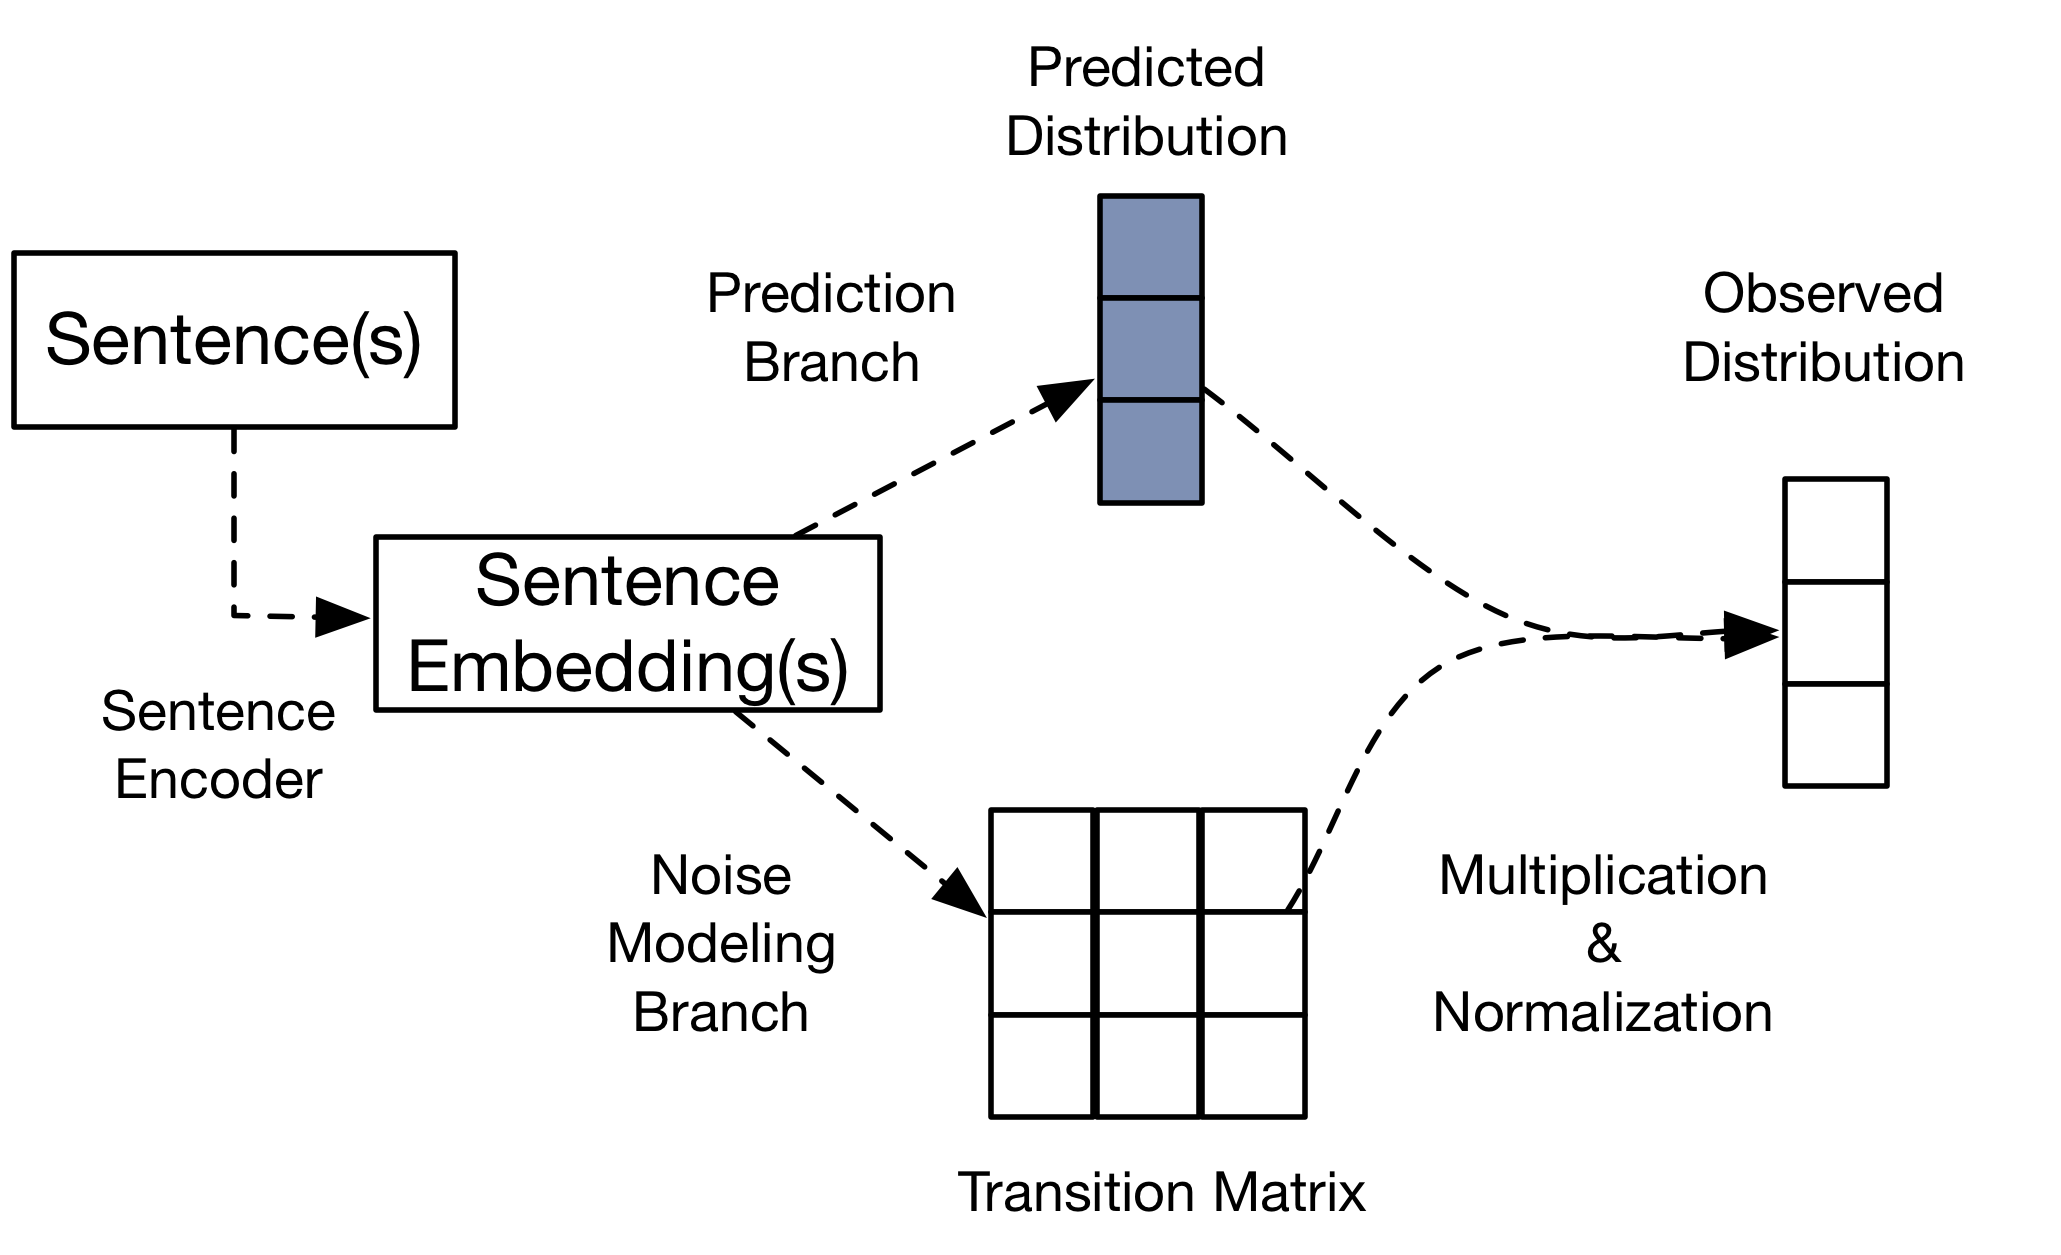
\includegraphics[width=8cm]{figures/denoise_framework.png}	
\caption{The architecture of our denoising model}
\label{fig: denoise_framework}
\end{center}
\end{figure}

The overview of our model is shown in Figure \ref{fig: denoise_framework}. First, the input sentence (or sentence bag) is passed to a sentence encoder to get sentence embedding(s). After that, the model is split into two branches. The prediction branch generates the predicted relation distribution $\mathbf{p}$ of the input sentence (or sentence bag). The noise modeling branch generates the transition matrix $\mathbf{T}$. Finally, the predicted distribution is multiplied by the transition distribution to generate the observed relation distribution $\mathbf{o}$. The predicted relation distribution $\mathbf{p}$ is the output of the model while the observed relation distribution $\mathbf{o}$ is used to simulate the relation assigned by distant supervision. In this way, the noise is modeled by the transition matrix and the real prediction is protected from the influence of the noise.

\subsection{Sentence Encoder}
\todo{add distance embedding}
Similar to previous researches in relation extraction, we also use the piecewise convolutional neural network (PCNN) model \cite{zeng2015distant} as our sentence encoder. The PCNN model first divides the input sentence into three pieces by the subject and the object. After that, it will apply convolutional neural network (CNN) to each piece to calculate the piece embedding. The final sentence embedding is the concatenation of the embeddings of the three pieces.

\subsection{Prediction Branch}
The prediction branch can be implemented by the prediction part of almost all the relation extraction neural network models. As for sentence level models, we use the settings of \cite{luo2016temporal}. Specifically, we first feed the sentence embedding to a full connection layer, and use softmax classifier for relation classification. As for bag level models, the key problem is how to aggregate the embeddings of each sentence in a bag. Similar to \cite{lin2016neural}, we experiment with two settings: average aggregation and attention aggregation. The average aggregation calculates the bag embedding $\mathbf{s}$ by averaging the embeddings of each sentence, and the resultant bag embedding is fed to a softmax classifier for relation classification. The attention aggregation method \cite{lin2016neural} calculates bag embeddings with respect to each relation. For example, the bag embedding with respect relation $j$ is:
\begin{equation}
\mathbf{s}_j = \sum_i^{n}{\alpha_{ij} \mathbf{x}_{i}}
\end{equation}
\begin{equation}
\alpha_{ij} = \frac{exp(\mathbf{x}_{i}^T \mathbf{Ar}_j))}{\sum_{i}{exp(\mathbf{x}_{i}^T \mathbf{Ar}_j)}}
\end{equation}
where and $\alpha_{ij}$ is the attention over sentence $i$ with respect to relation $j$, $\mathbf{A}$ is a diagonal matrix and $\mathbf{r_j}$ is the randomly initialized embedding of relation $j$. The resultant bag embedding is fed to a softmax classifier to predict the probability of relation $j$.

\subsection{Noise Modeling Branch}
Parallel to the prediction branch, the noise modeling branch calculates a transition matrix dynamically for each sentence (or sentence bag) to model its noise pattern.

\paragraph{Sentence Level Transition Matrix}
As for sentence level models, the sentence embedding $\mathbf{x}$ is passed to another full connection layer to obtain the sentence embedding $\mathbf{x}_n$ used specifically for the noise branch. After that, the transition matrix $\mathbf{T}$ is calculated using a softmax classifier:
\begin{equation}
T_{ij} = \frac{exp({(\mathbf{w}_t^{ij})^T \mathbf{x}_n + b_t})}{\sum_{j=1}^{|\mathbb{C}|}{exp({(\mathbf{w}_t^{ij})^T \mathbf{x}_n + b_t}})}
\end{equation}
where $T_{ij}$ is the conditional probability that this sentence is labeled as relation $j$ by distant supervision given the true relation is $i$, $\mathbf{w}_t^{ij}$ is the weight vector for this situation, $b_t$ is a scalar bias and $|\mathbb{C}|$ is the number of relations.

\paragraph{Bag Level Transition Matrix}
As for bag level models, we first use the attention mechanism to calculate the bag embedding with respect to each relation:
\begin{equation}
\mathbf{s}_{j} = \sum_i^{n}{\alpha_{ij} \mathbf{x}_{i}}
\end{equation}
\begin{equation}
\alpha_{ij} = \frac{exp(\mathbf{x}_i^T \mathbf{r}_t^j)}{\sum_i^n{exp(\mathbf{x}_i^T \mathbf{r}_t^j)}}
\end{equation}
where $\mathbf{s}_j$ is the bag embedding with respect to relation $j$, $\mathbf{x}_i$ is the embedding of sentence $i$, $\alpha_{ij}$ is the attention value and $\mathbf{r}_t^j$ is another randomly initialized embedding of relation $j$ used specifically for noise modeling branch.

Then the transition matrix $\mathbf{T}$ is calculated by:
\begin{equation}
T_{ij} = \frac{exp({(\mathbf{r}_t^j)^T \mathbf{s}_i + b_t})}{\sum_{j=1}^{|\mathbb{C}|}{exp((\mathbf{r}_t^j)^T \mathbf{s}_i + b_t})}
\end{equation}
where $\mathbf{s}_i$ is the bag embedding with respect to relation $i$, $\mathbf{r}_t^j$ is the embedding of relation $j$ mentioned above, and $b_t$ is a scalar bias.

Note that the softmax function guarantees that each row of the transition matrix $\mathbf{T}$ sums to 1 in both sentence level and bag level models. Here $T_{ij}$ represents the conditional probability that the relation labeled by distant supervision is $j$ given the true relation is $i$.


\subsection{Observed Relation Distribution}
Given the predicted relation distribution $\mathbf{p}$ calculated by the prediction branch, and the transition matrix $\mathbf{T}$ calculated by the noise modeling branch, the observed relation distribution $\mathbf{o}$ is calculated by:
 \begin{equation}
\mathbf{o} = \mathbf{T}^T \bm\cdot \mathbf{p}
 \end{equation}
 \begin{equation}
 \label{norm_o}
 o_i = \frac{o_i}{\sum_i{o_i}}
 \end{equation}
 where $\bm\cdot$ represents dot product and Equation \ref{norm_o} normalizes the elements of $\mathbf{o}$ so that $\sum_i{o_i}=1$

Different from previous works that use the predicted relation distribution $\mathbf{p}$ to directly match the relation labeled by distant supervision. We instead use $\mathbf{o}$ to match the relation assigned by distant supervision. In this way, we can model the procedure of how the noisy label is produced and thus protect our prediction $\mathbf{p}$ from the influence of the noise.

Note that the noise modeling branch and $\mathbf{o}$ is only used in the training phase. In the test phase, we only use the prediction brach and take the predicted relation distribution $\mathbf{p}$ as our output.

\section{Training Procedure}
Note that if we apply the transition matrix model directly to the training data, there is no incentive for the predicted relation distribution $\mathbf{p}$ to model the true relation distribution, instead it will probably be treated as a normal hidden layer. In this section, we show how to combine the curriculum learning framework and a novel normalization strategy to solve this problem. We describe the training procedure in the situation with and without the prior knowledge of the data quality.

\subsection{Curriculum Learning over Dataset}
\todo{describe the curriculum learning for bag level methods in experiment part}
The basic idea of curriculum learning is simple: start with the easiest aspect of a task, and level up the difficulty gradually.

The most straight forward way to build a curriculum is by controlling the training data. If we have both reliable and unreliable data, we can first train the prediction branch on the reliable data for $t_1$ epochs so that the prediction branch will have the basic classification ability. Then we add the unreliable data as well as the noise modeling branch. In this way, the prediction branch will already possess the tendency to predict true relation distribution before exposed to noisy data.

Specifically, in the dataset of \cite{luo2016temporal}, we have three subsets with decreasing reliability. We first train the prediction branch on the reliable subset for $t_1$ epochs. After that, we add the less reliable subset and the most unreliable subset consecutively and train for $t_2$ and $t_3$ epochs respectively (for simplicity, here we set $t_1=t_2=t_3$).

\subsection{Trace Normalization}
The curriculum learning method above only works when we know which data are reliable. Here we introduce how to use trace normalization to control the behavior of the transition matrix and how to use this method to build a more general curriculum in the next section.

Intuitively, if the noise is small, the transition matrix $\mathbf{T}$ will tend to become an identity matrix. Therefore, we can utilize our prior knowledge of the data quality by controlling the similarity between $\mathbf{T}$ and identity matrix. In the situation where we do not know which data are reliable, we can first force the transition matrix to be similar to identity matrix until the prediction branch is roughly trained. Then by gradually relax the constraint, the model will gradually learn to model the noise in the dataset.

Specifically, since each row of $\mathbf{T}$ sums to 1, the similarity between the transition matrix and the identity matrix can be represented by the trace of the transition matrix $\mathbf{T}$. The larger the $trace(\mathbf{T})$ is, the smaller the elements that do not lie in the diagonal are, and the similar the transition matrix $\mathbf{T}$ is to identity matrix.

Since we have the prior knowledge of the quality of the three subsets of the dataset of Luo et.al, we can further use three hyper-parameters $\{\beta_1, \beta_2, \beta_3\}$ to control the $trace(\mathbf{T})$ of the three subsets. For reliable subset, we want $trace(\mathbf{T})$ to be large (negative $\beta_1$) so that the element values of $\mathbf{T}$ will be centralized to the diagonal. As for unreliable subsets, we want the $trace(\mathbf{T})$ to be small (positive $\beta_2$ and $\beta_3$) so that the element values of their transition matrices will be diffusive. Note that this method only works for sentence level models, since reliable sentences and unreliable ones are all aggregated into a sentence bag in bag level models and therefore we can not determine which bag is reliable. and which is not. We use cross entropy as our basic loss function, and the loss function of the sentence level model is defined as follows:

\begin{equation}
\begin{aligned}
J(\theta)=\sum_{i=1}^3{\sum_{j=1}^{N_i}{-log(o_{ijy_{ij}})}} + \beta_i trace(\mathbf{T}_{ij})
\end{aligned}
\end{equation}
where $\theta$ represents all the parameters in our model, $i$ is the index of the three subsets, $j$ is the index of sentence, $\mathbf{T}_{ij}$ is the transition matrix of sentence $s_{ij}$, $y_{ij}$ is the relation assigned by distant supervision for sentence $s_{ij}$, and $o_{ijy_{ij}}$ is the probability that the observed relation for sentence $s_{ij}$ is $y_{ij}$.

\subsection{Curriculum Learning over Noise Modeling Strength}
As for bag level models, and in the situation where we do not have prior knowledge of the data quality, we can build a curriculum by controlling our expectation for the model to model the noise. Specifically, the loss function is defined as follows:

\begin{equation}
\begin{aligned}
J(\theta)	&=\sum_{i=1}^N{-(\alpha log(o_{iy_{i}}) + (1-\alpha) log(p_{iy_{i}}))} \\
&+ \beta trace(\mathbf{T}_{i})
\end{aligned}
\end{equation}
where $0\le\alpha\le1$, $y_i$ is the relation assigned by distant supervision for sentence $s_i$, $o_{iy_{i}}$ and $p_{iy_{i}}$ is the probability that the observed and predicted relation for setnence $s_i$ is $y_i$. \todo{polish the statement before} Instead of only using the observed relation distribution $\mathbf{o}$ to simulate the relation labeled by distant supervision, we use the linear combination of the cross entropy of both the observed relation distribution $\mathbf{o}$ and the predicted relation distribution $\mathbf{p}$.

At the start of the training, we set $\alpha=1$ and $\beta<0$, which means we do not expect the model to model the noise (easy part of the problem). As the training proceeds, the prediction branch gradually learns the basic prediction ability. Therefore, we decrease $\alpha$ and the absolute value of $\beta$ by $d$ every $\tau$ epochs to gradually lead the model to learn to model the noise.

\subsection{Constraint Transition Matrix}
Recall that the bag level noise mainly consists of false negative and false positive, but our transition matrix also has the ability to model the confusion among positive relations. To prevent overfitting and make the model concentrate on the false negative and false positive noise, we restrict the transition matrix for bag level models so that only the diagonal, the first column and the first row of the transition matrix do not equal to zero (assume the index of \emph{no-relation} is 0). 